\section{Evaluation}\label{s:eval}

\FYI{

# Ext4
-
- Score

# F2FS
- Score

# Fragmentation on FDP?

}

% Evaluation environment
\FYI{
# Host configuration

# Lines of code

}


\begin{comment}
초반 - 실험 환경 설명 Eval Setup

들어가야 하는 내용 : 
  1. 실제로 노화가 영향을 주나? => latency과 dynamic score를 비교하며, dynamic score과 반비례하여 latency가 증가한다.
								 왜 이런 결과가 나오는지? fragmentation 때문인데, 이걸 그림과 대조하며 설명.
								 근데 어떤 그림을 사용해야 할지 고민됨. 

  2. dump하는데 필요한 저장공간 => 그래서 update된 storage부분만 snapshot뜨기로 함. => 이건 어느정도?
 	 전체 storage를 dump vs update된 storage만 dump 했을 때의 시간 차이
	 => 큰 차이는 없고 데이터 배치에 따라 결과값이 달라짐. 
	 => 굳이 따지면 save는 update된 storage만 dump하는게 조금떠 빠르고 load는 느리게 관측됨
	 => 이 이유는 load할때에는 기존에 가지고 있는 데이터를 지워야 하는데, 이 지우는 것에서 latency가 발생하는 것으로 보임.
	 => save의 경우에는 데이터를 읽어오는데, update된 data만 dump 뜨는 것은, 어차피 전체 storage를 봐야하는것은 original한 방법도 동등.
	 하지만 original방법은 데이터를 저장하는 latency도 발생하지만, update된 data만 저장하는 버전은 사용하지 않는 data를 save하는 latency가 없음.


\end{comment}
%  Git workload
The Git aging benchmark\cite{conway:login17,senescence:fast17} can measure aging in a real-world environment that people commonly use.
Git is a distributed version control system that allows synchronization of source code changes.
It generates workloads by simulating developers working on collaborative projects using Git.
Experiments are conducted using the git pull command, which creates new source files, deletes old files, or modifies files. During this process, Git maintains its internal data structure, leading to filesystem aging.
To measure the extent of aging, multiple git pull commands can be executed, and latency can be measured through reads using grep.

% Setup

\begin{figure}[t]
    \centering
    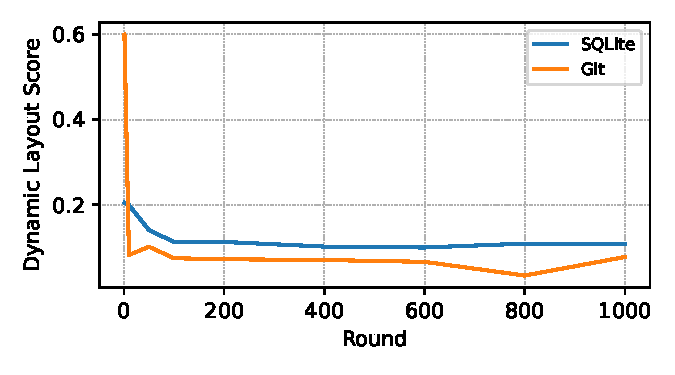
\includegraphics[width=0.95\columnwidth]{graphs/py_graph/dynamic}
    \caption{Dynamic}
    \label{f:dynamic}
\end{figure}

\begin{figure}[t]
    \centering
    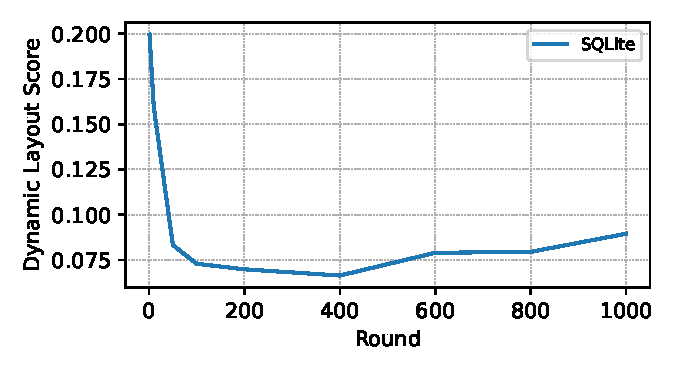
\includegraphics[width=0.95\columnwidth]{graphs/py_graph/dynamic-f2fs}
    \caption{F2FS dynamic score}
    \label{f:f2fs_dynamic_score}
\end{figure}


\begin{figure}[t]
    \centering
    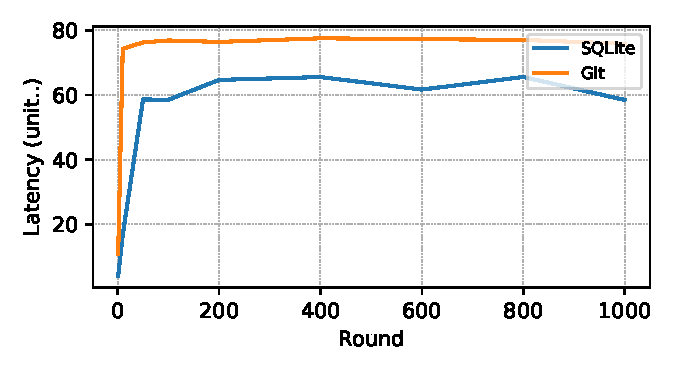
\includegraphics[width=0.95\columnwidth]{graphs/py_graph/latency}
    \caption{Latency}
    \label{f:latency}
\end{figure}

\begin{figure}[t]
    \centering
    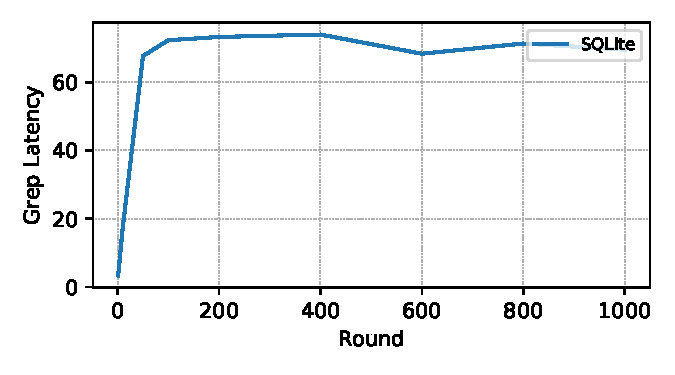
\includegraphics[width=0.95\columnwidth]{graphs/py_graph/latency-f2fs}
    \caption{F2FS latency}
    \label{f:f2fs_latency}
\end{figure}


\begin{figure}[t]
    \centering
	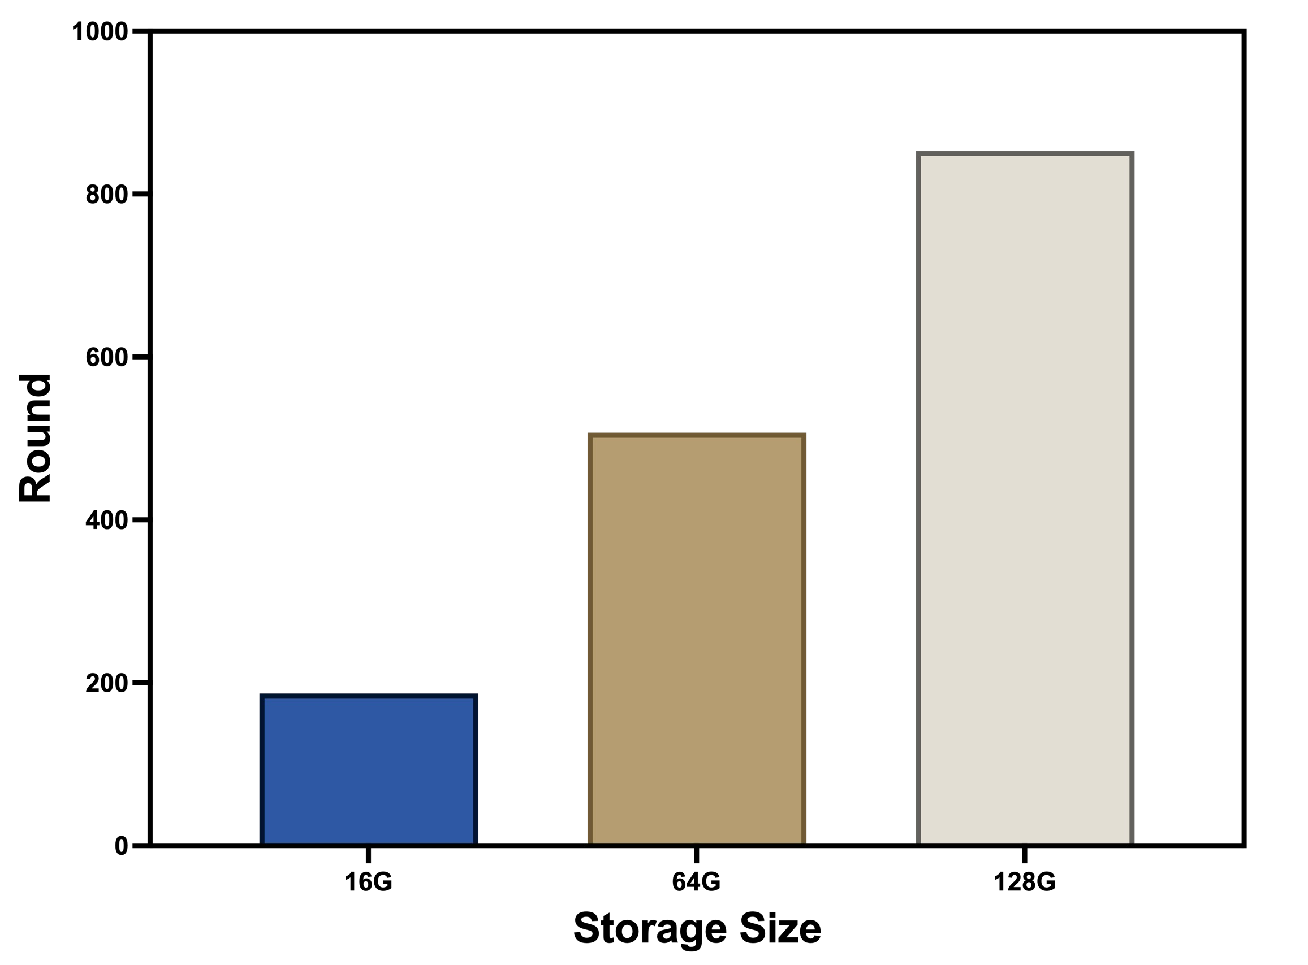
\includegraphics[width=0.95\columnwidth]{aging_duration}
    \caption{Aging duration}
    \label{f:aging_duration}
\end{figure}

\begin{figure}[t]
    \centering
	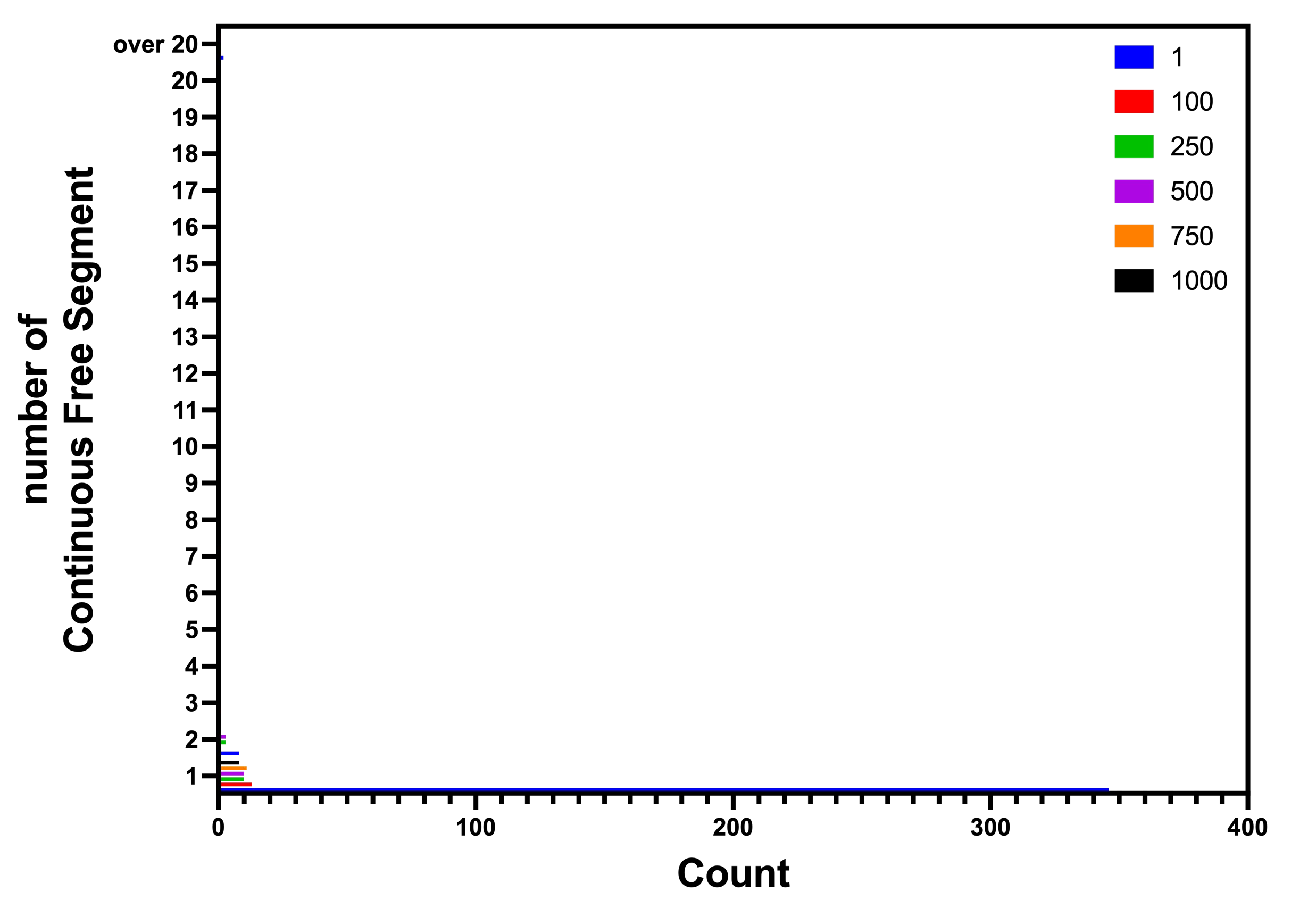
\includegraphics[width=0.95\columnwidth]{continuous_free_segment_fsfs}
	\caption{}
	\label{f:}
\end{figure}

\begin{figure}[t]
    \centering
	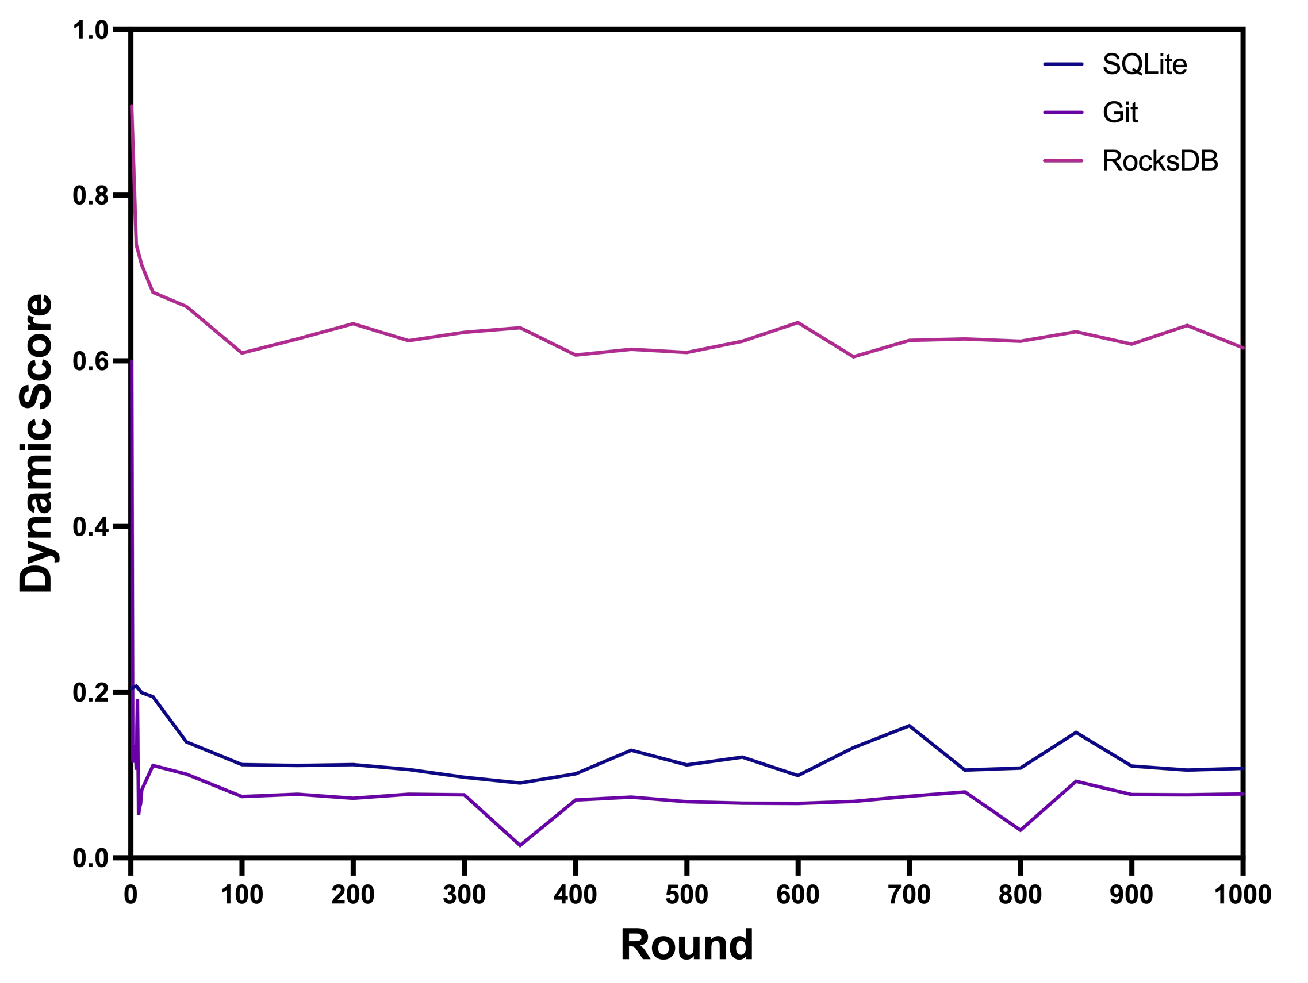
\includegraphics[width=0.95\columnwidth]{ext4_dynamic}
	\caption{}
	\label{f:}
\end{figure}

\begin{figure}[t]
    \centering
	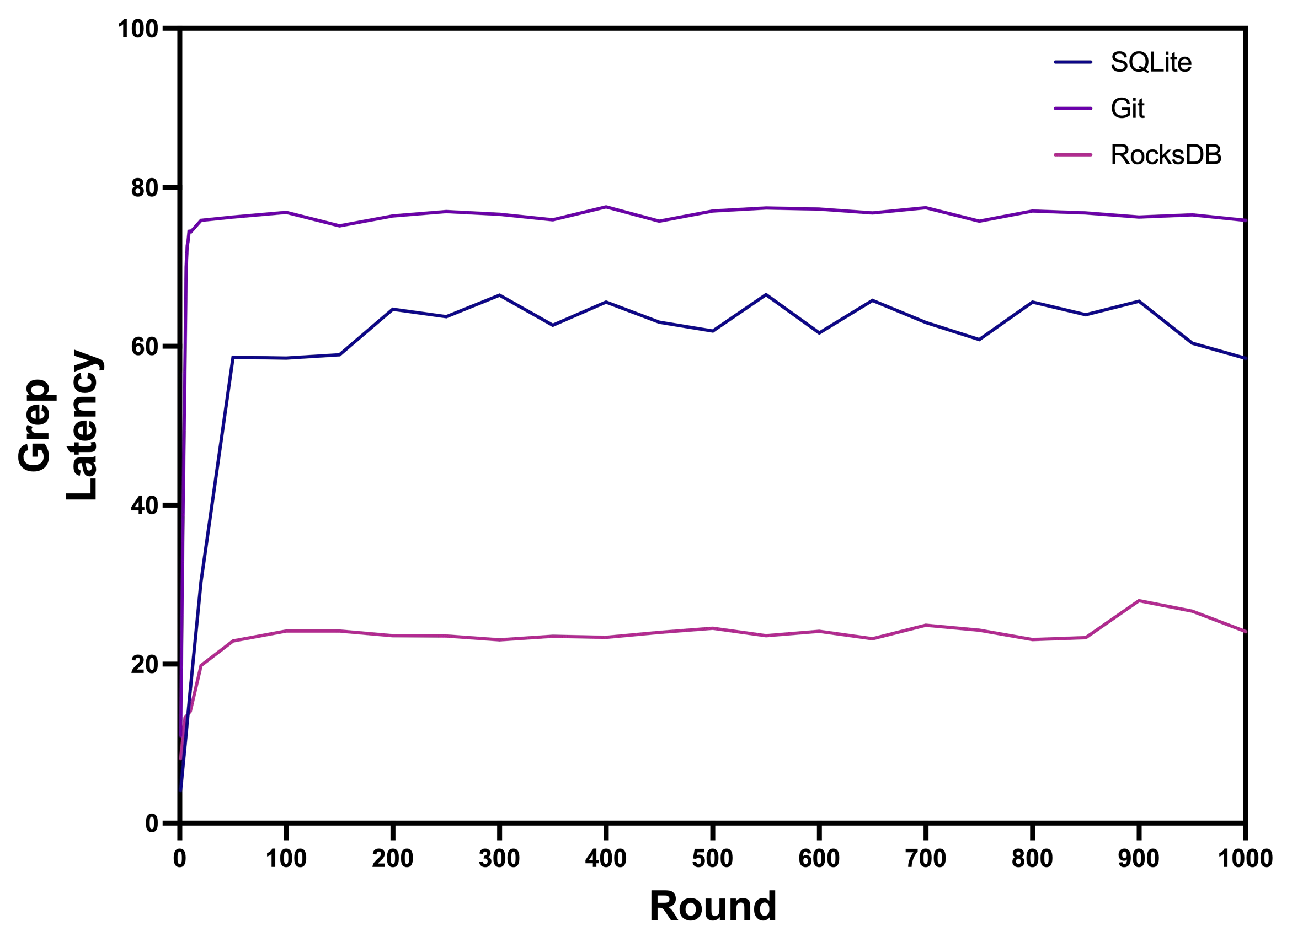
\includegraphics[width=0.95\columnwidth]{ext_latency}
	\caption{}
	\label{f:}
\end{figure}

\begin{figure}[t]
    \centering
	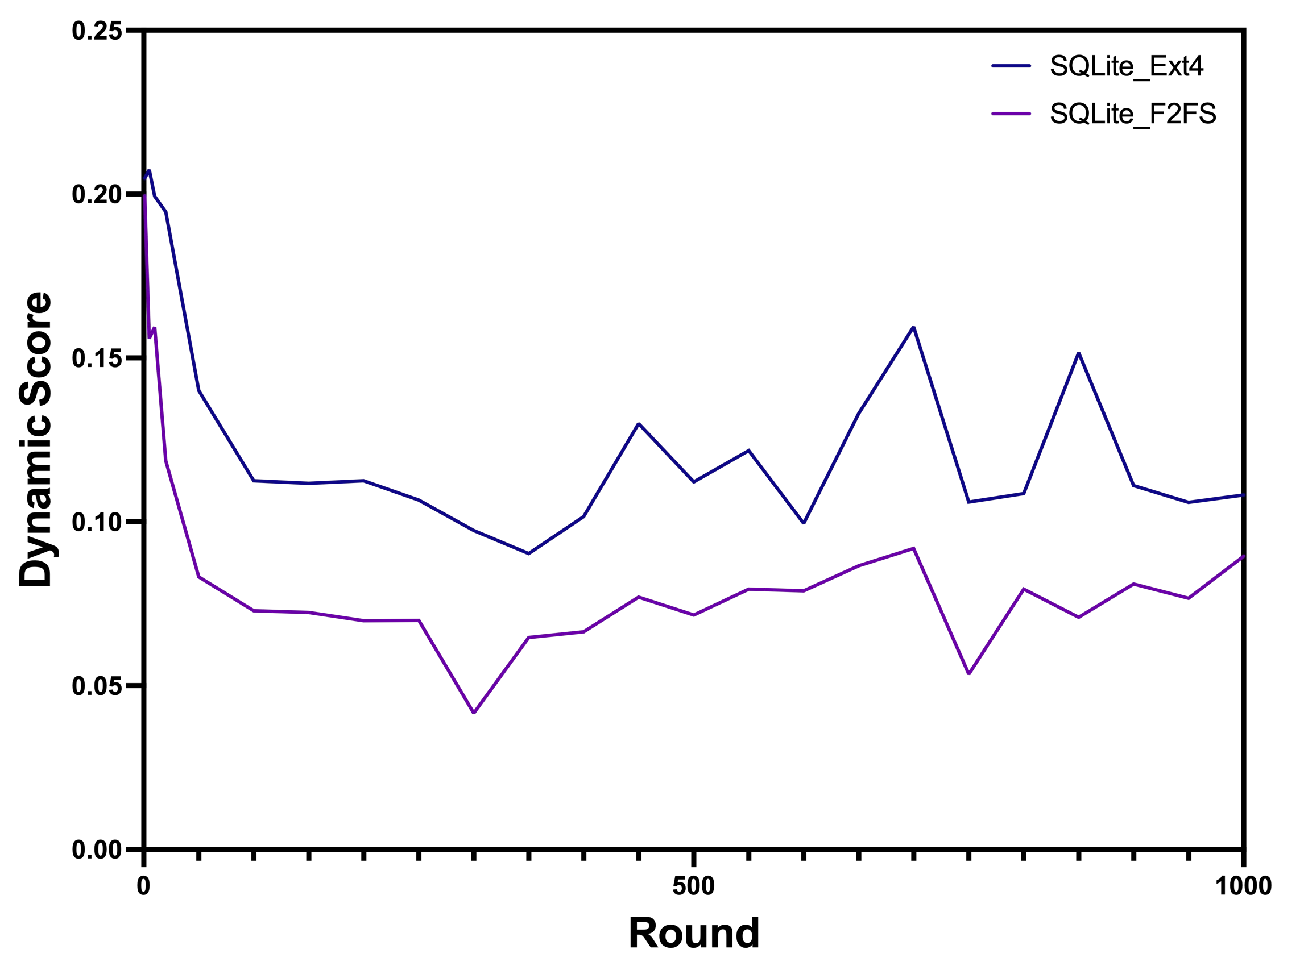
\includegraphics[width=0.95\columnwidth]{f2fs_vs_ext4_dynamic}
	\caption{}
	\label{f:}
\end{figure}

\begin{figure}[t]
    \centering
	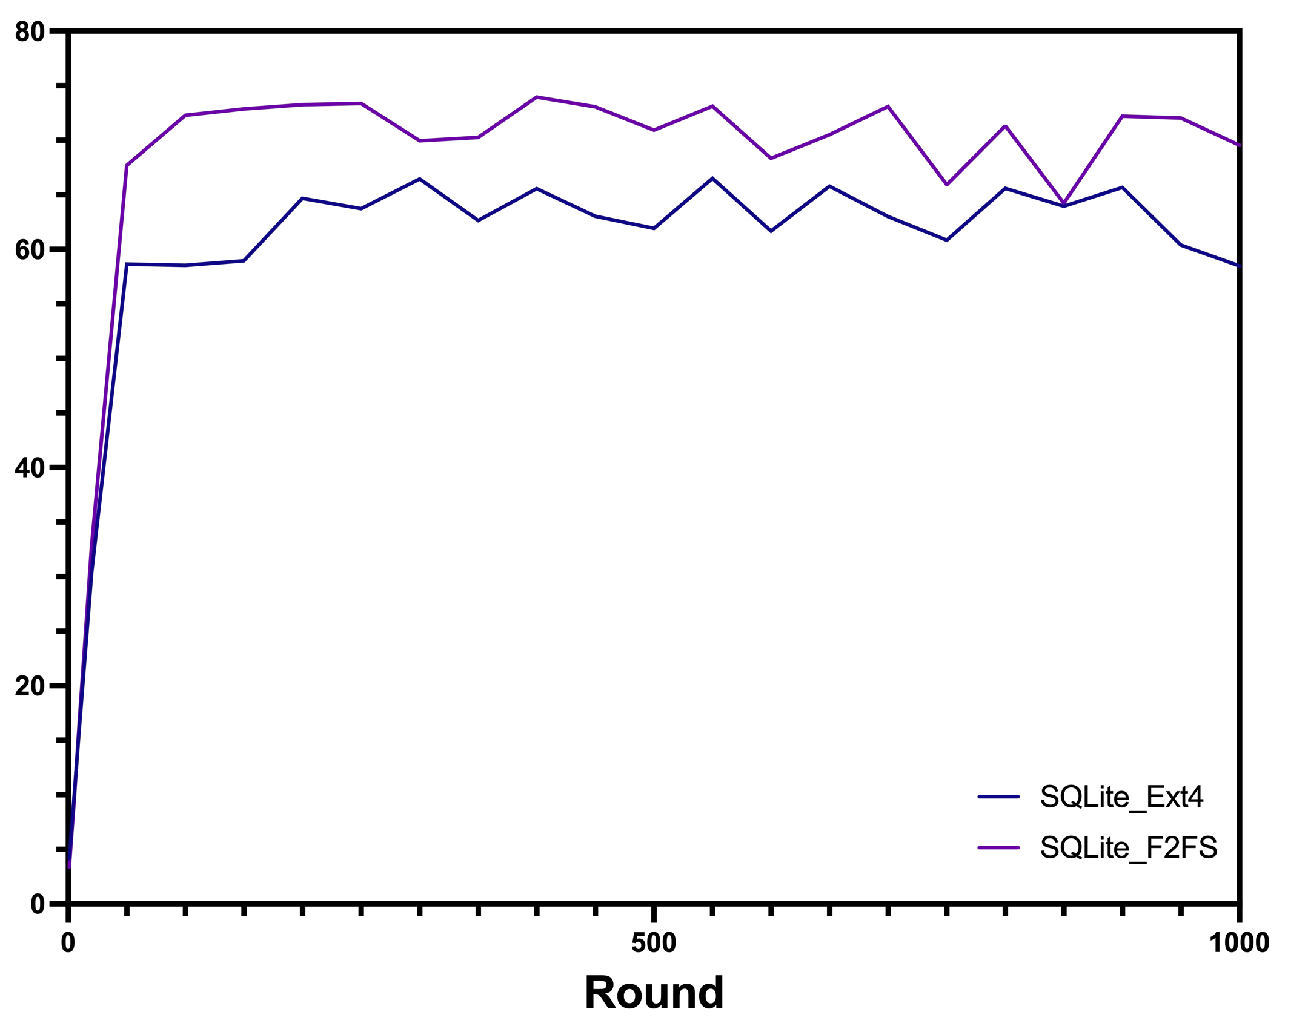
\includegraphics[width=0.95\columnwidth]{f2fs_vs_ext4_latency}
	\caption{}
	\label{f:}
\end{figure}

\begin{figure}[t]
    \centering
	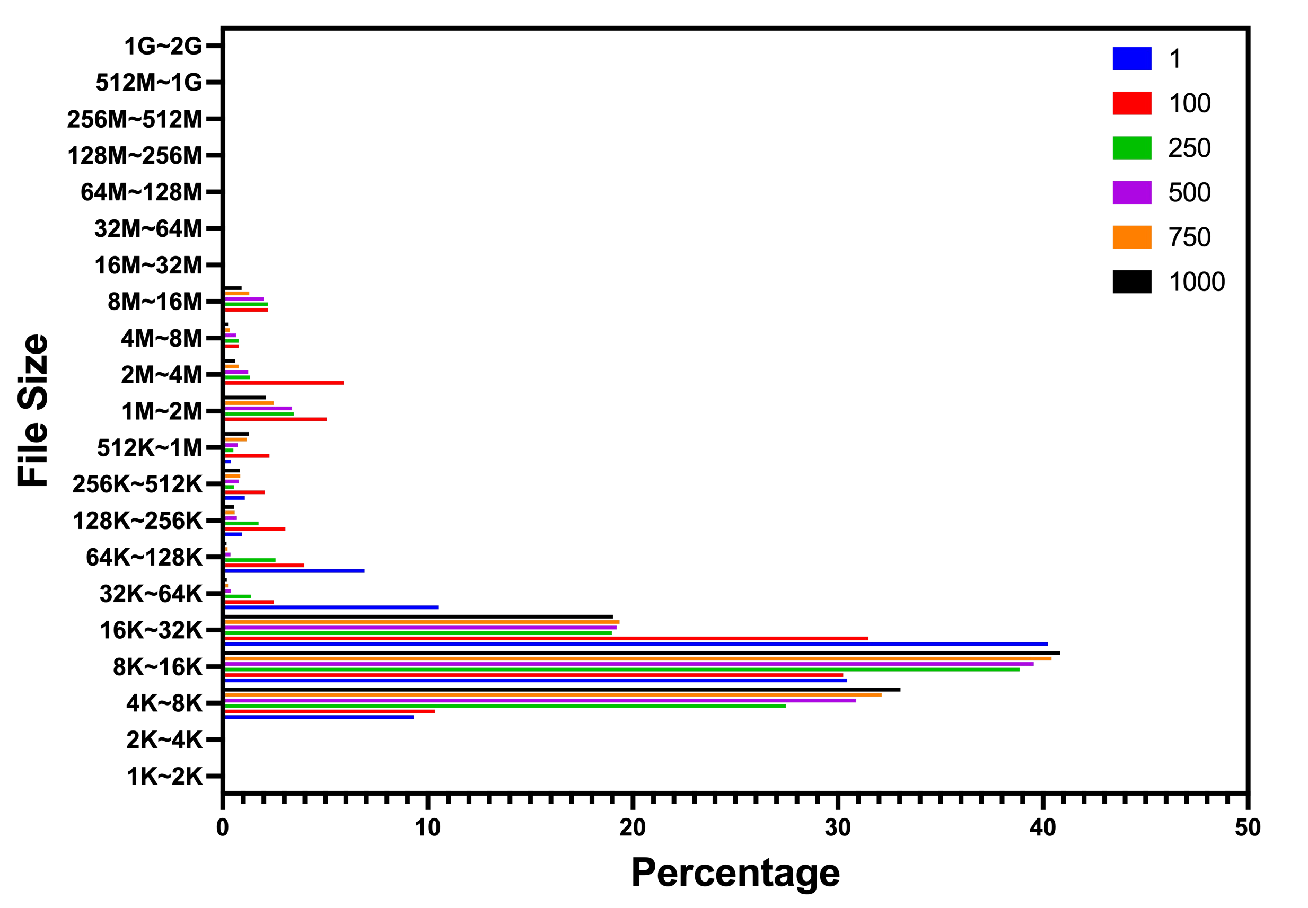
\includegraphics[width=0.95\columnwidth]{file_block_ext4}
	\caption{}
	\label{f:}
\end{figure}

\begin{figure}[t]
    \centering
	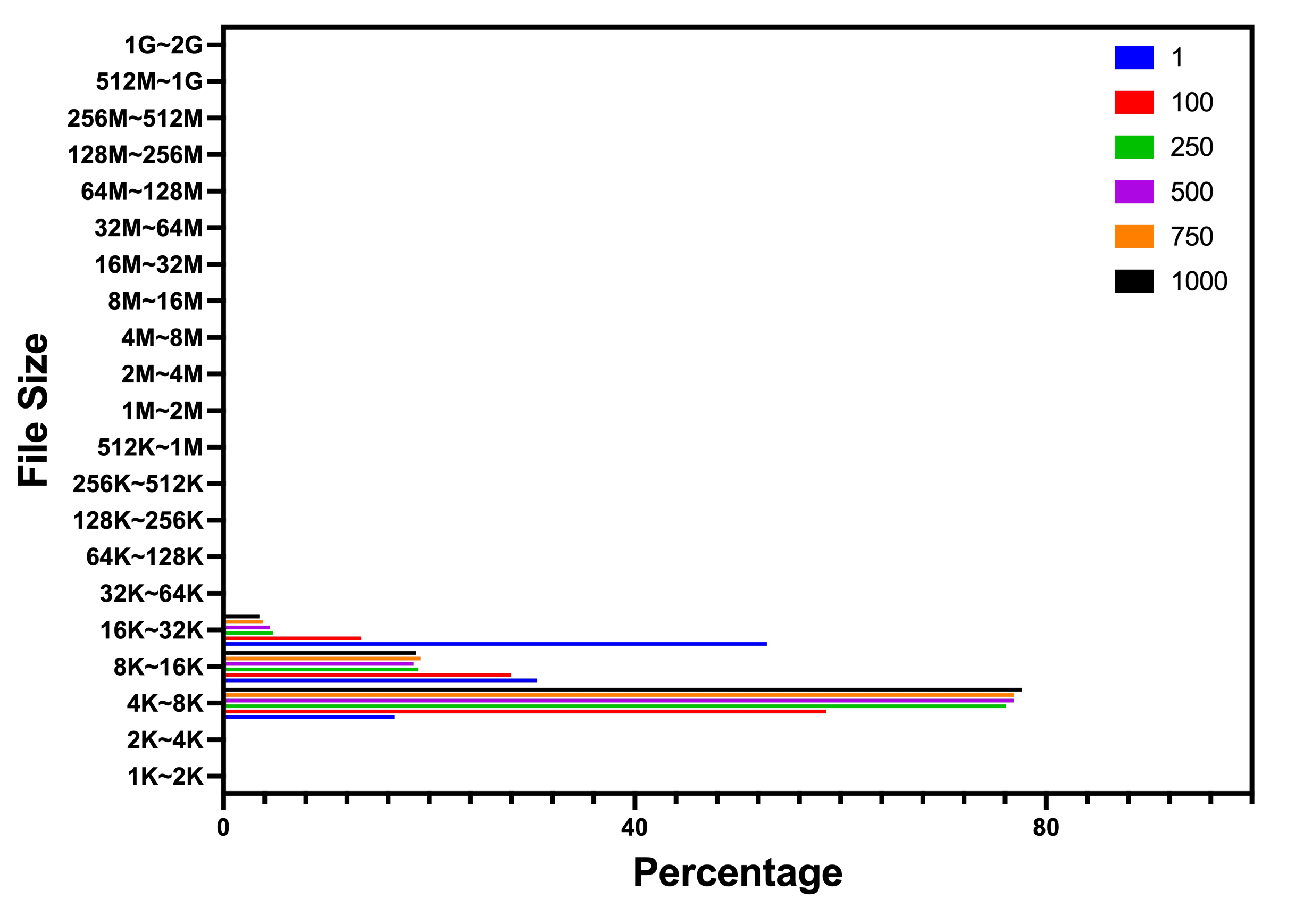
\includegraphics[width=0.95\columnwidth]{file_block_f2fs}
	\caption{}
	\label{f:}
\end{figure}

\begin{figure}[t]
    \centering
	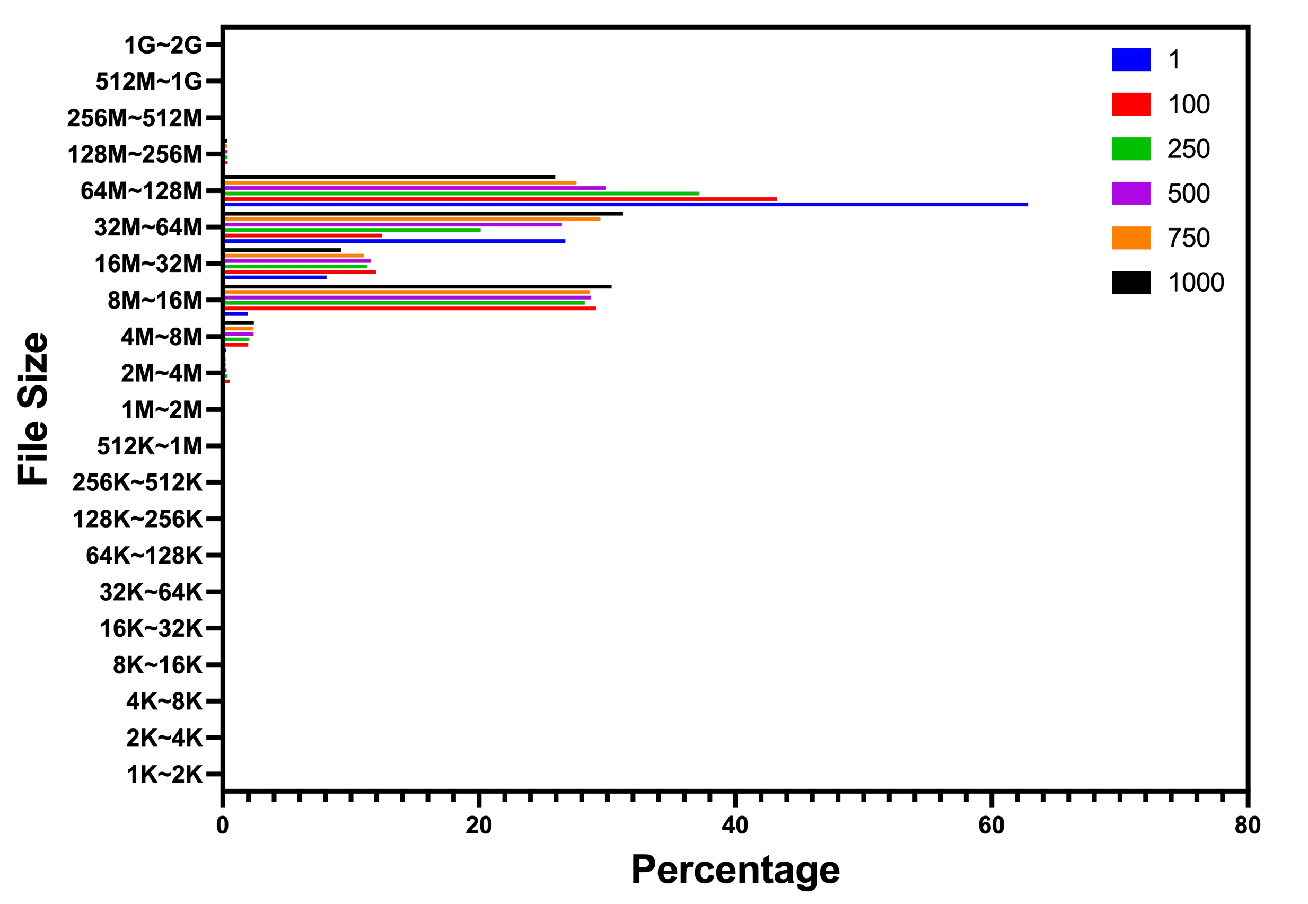
\includegraphics[width=0.95\columnwidth]{file_block_rocksdb}
	\caption{}
	\label{f:}
\end{figure}

\begin{figure}[t]
    \centering
	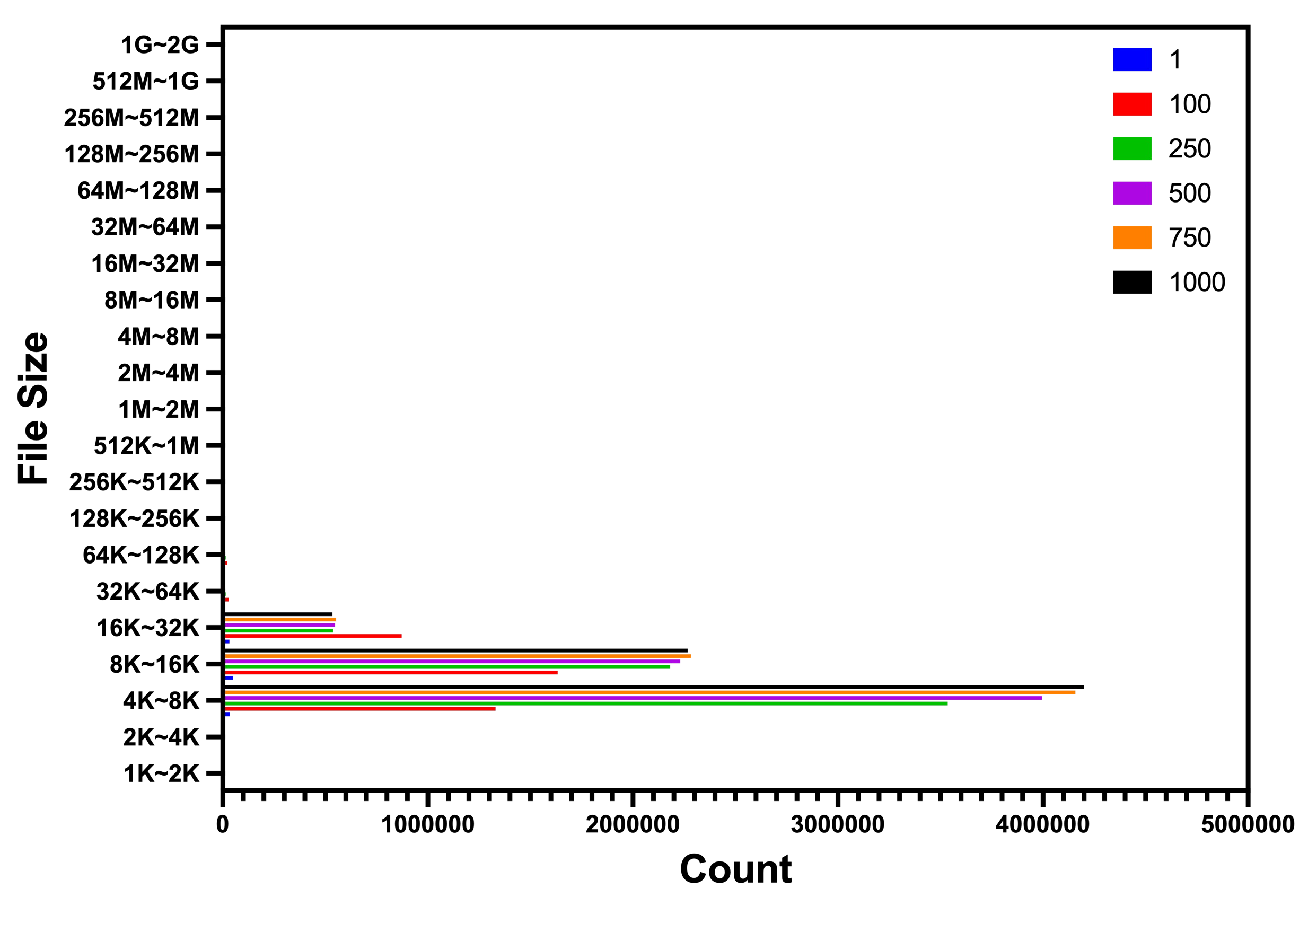
\includegraphics[width=0.95\columnwidth]{file_extents_ext4}
	\caption{}
	\label{f:}
\end{figure}

\begin{figure}[t]
    \centering
	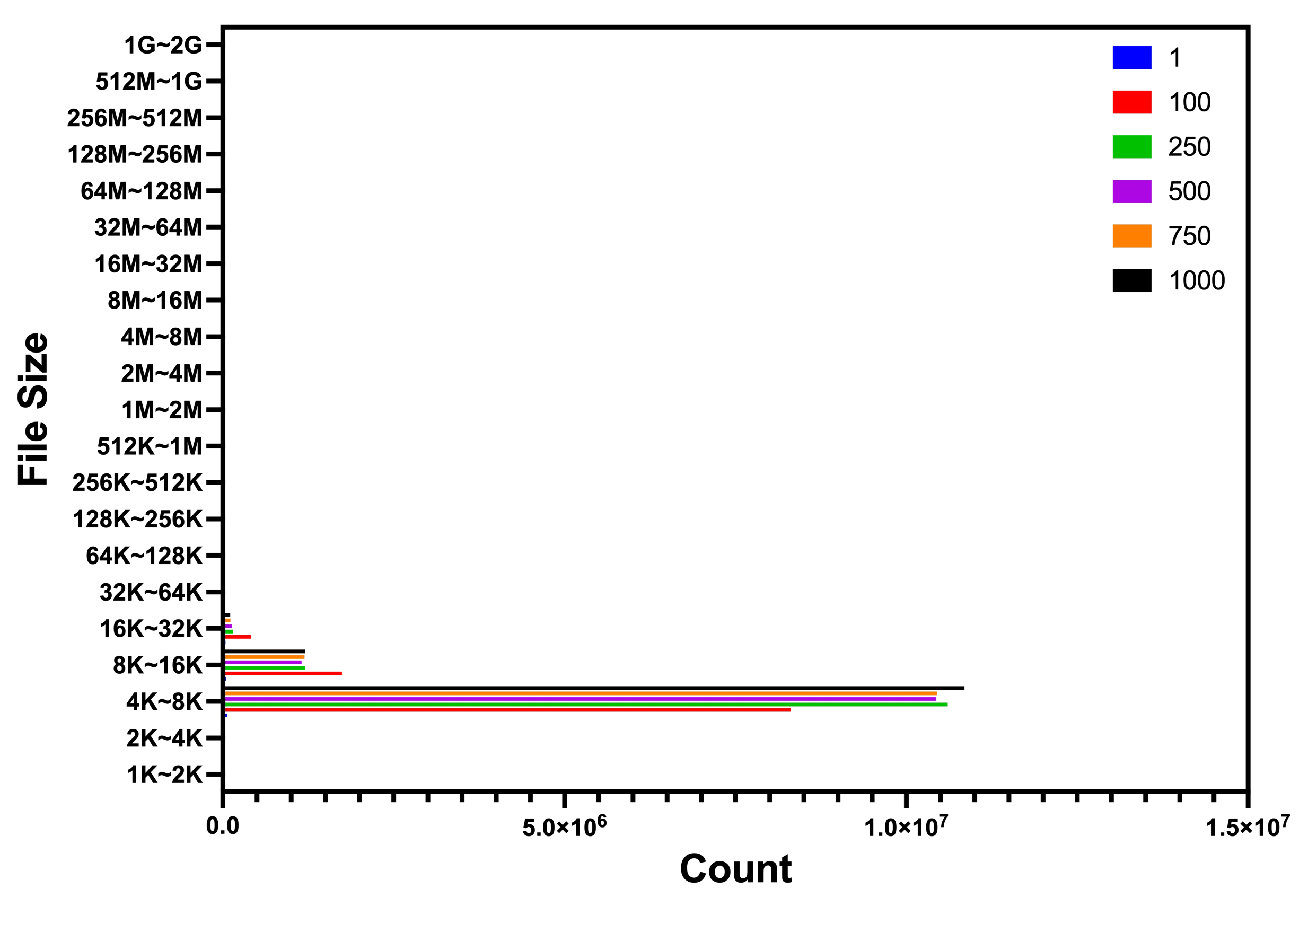
\includegraphics[width=0.95\columnwidth]{file_extents_f2fs}
	\caption{}
	\label{f:}
\end{figure}

\begin{figure}[t]
    \centering
	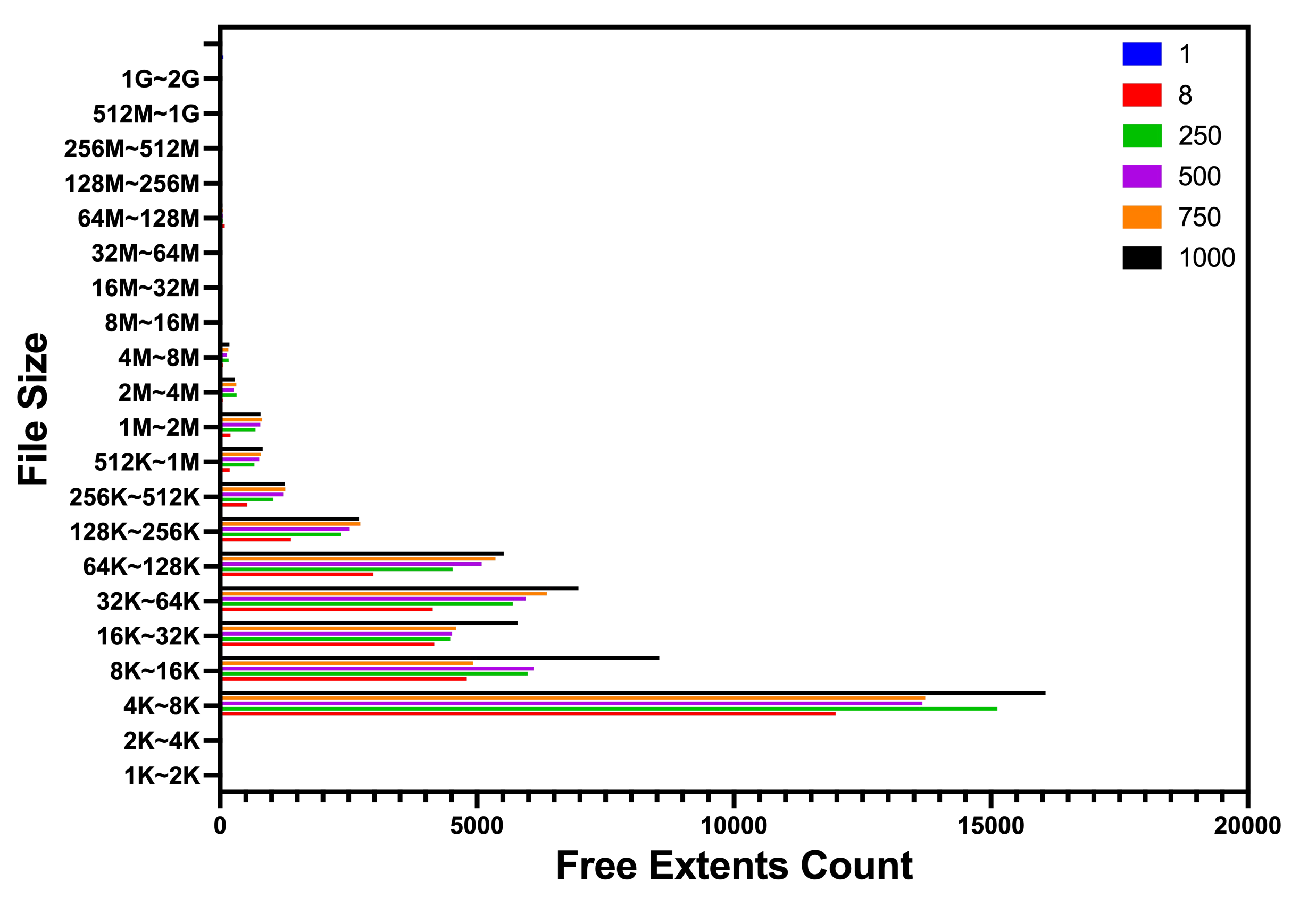
\includegraphics[width=0.95\columnwidth]{file_extents_git}
	\caption{}
	\label{f:}
\end{figure}

\begin{figure}[t]
    \centering
	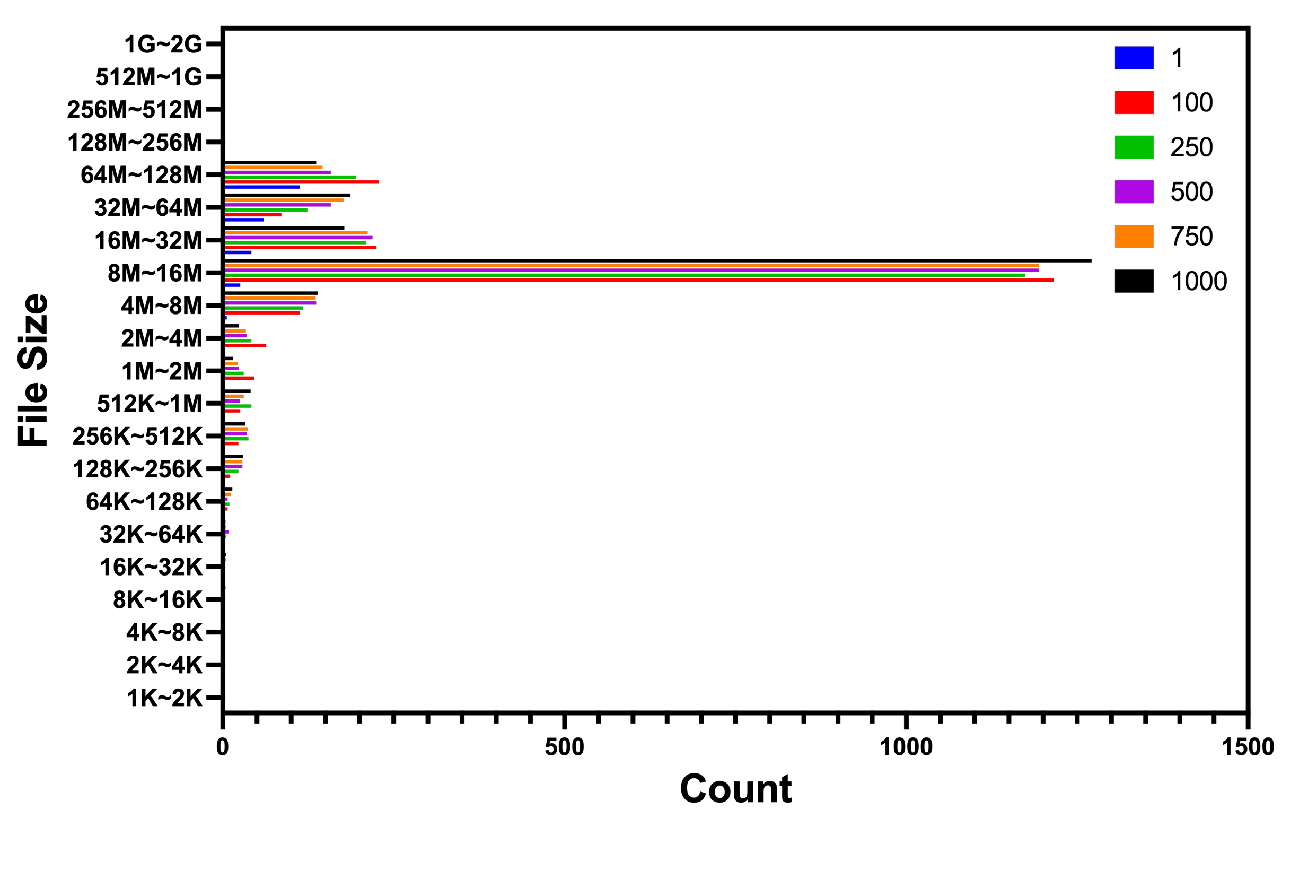
\includegraphics[width=0.95\columnwidth]{file_extents_rocksdb}
	\caption{}
	\label{f:}
\end{figure}

\begin{figure}[t]
    \centering
	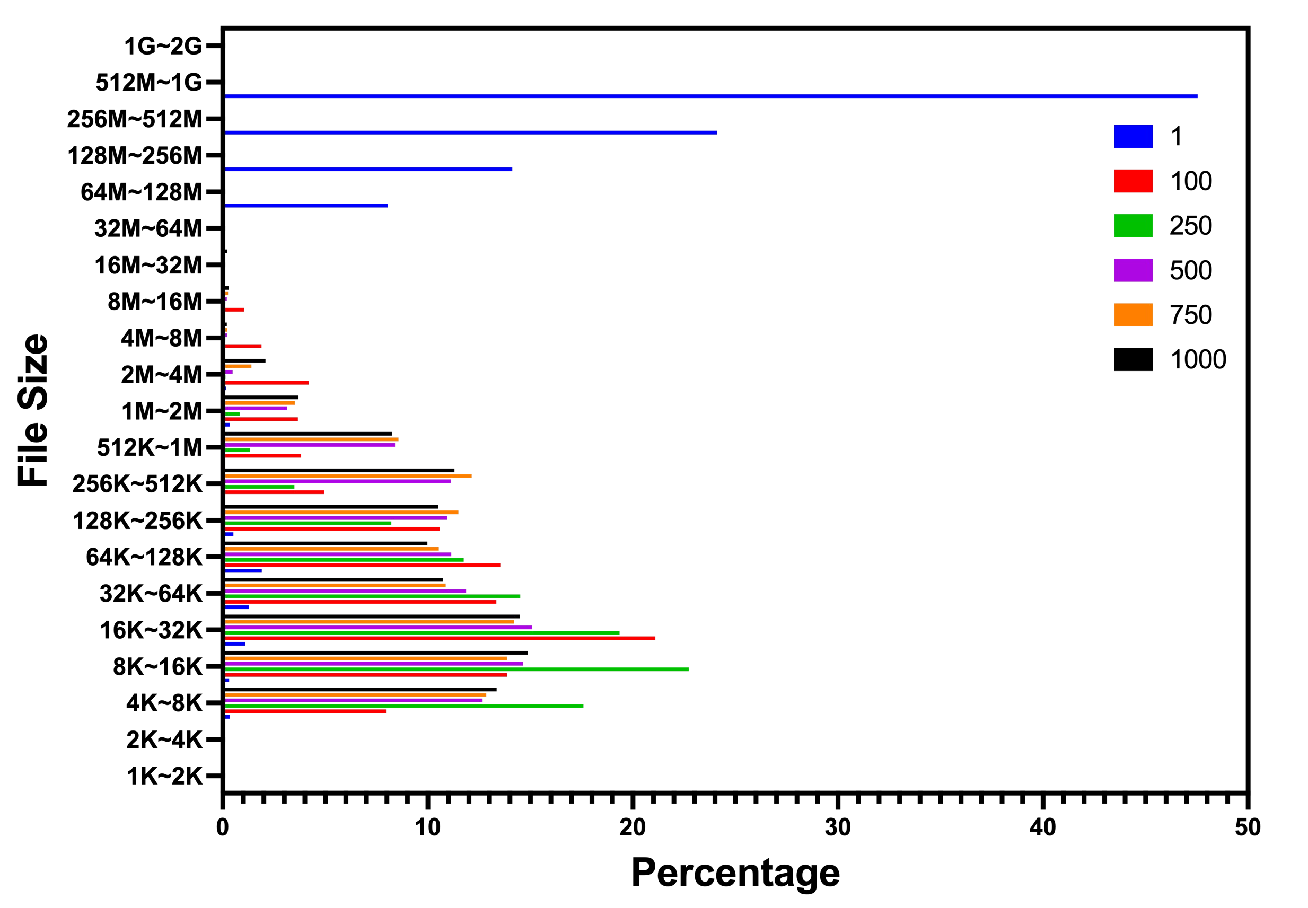
\includegraphics[width=0.95\columnwidth]{free_block_ext4}
	\caption{}
	\label{f:}
\end{figure}

\begin{figure}[t]
    \centering
	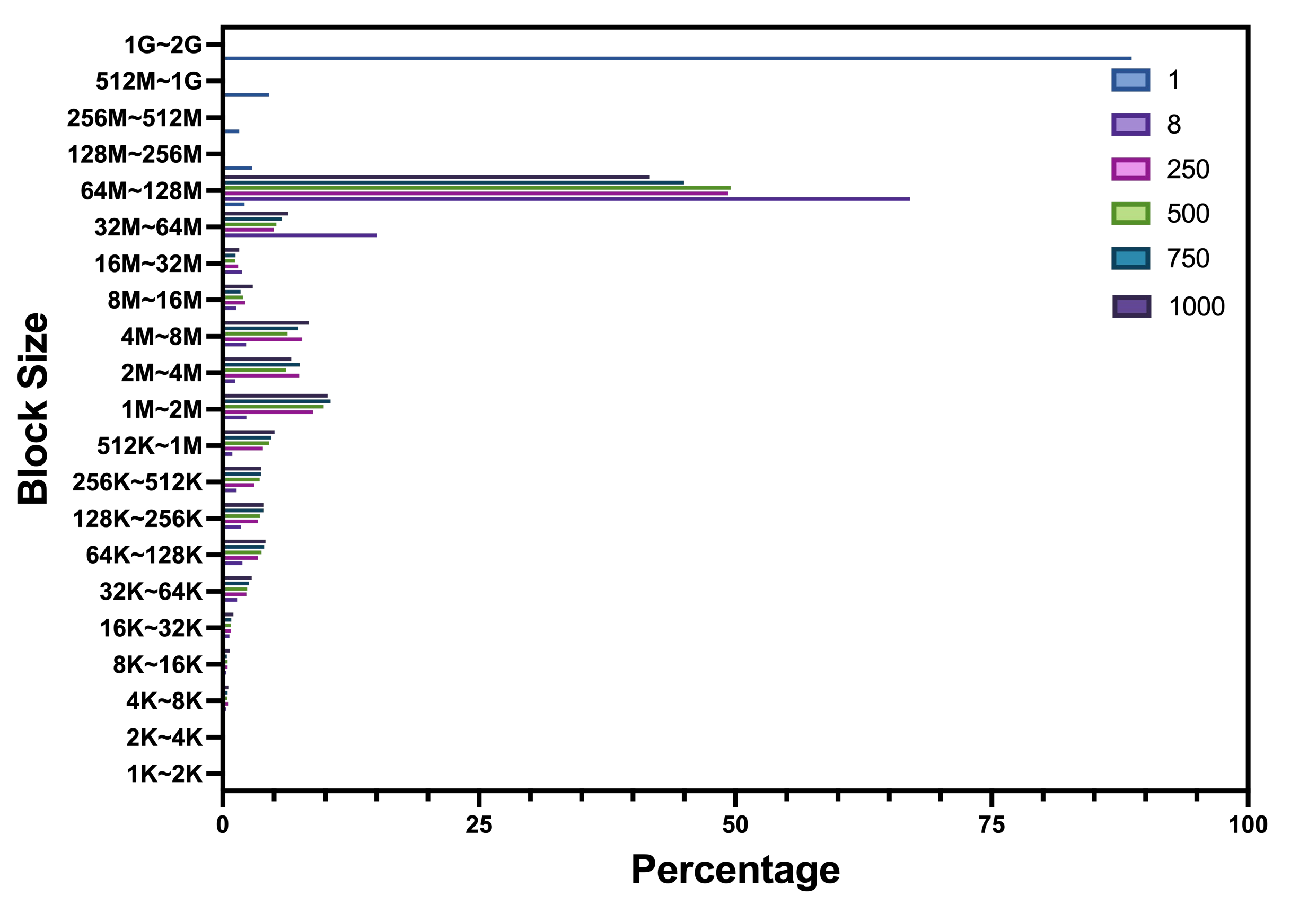
\includegraphics[width=0.95\columnwidth]{free_block_git}
	\caption{}
	\label{f:}
\end{figure}

\begin{figure}[t]
    \centering
	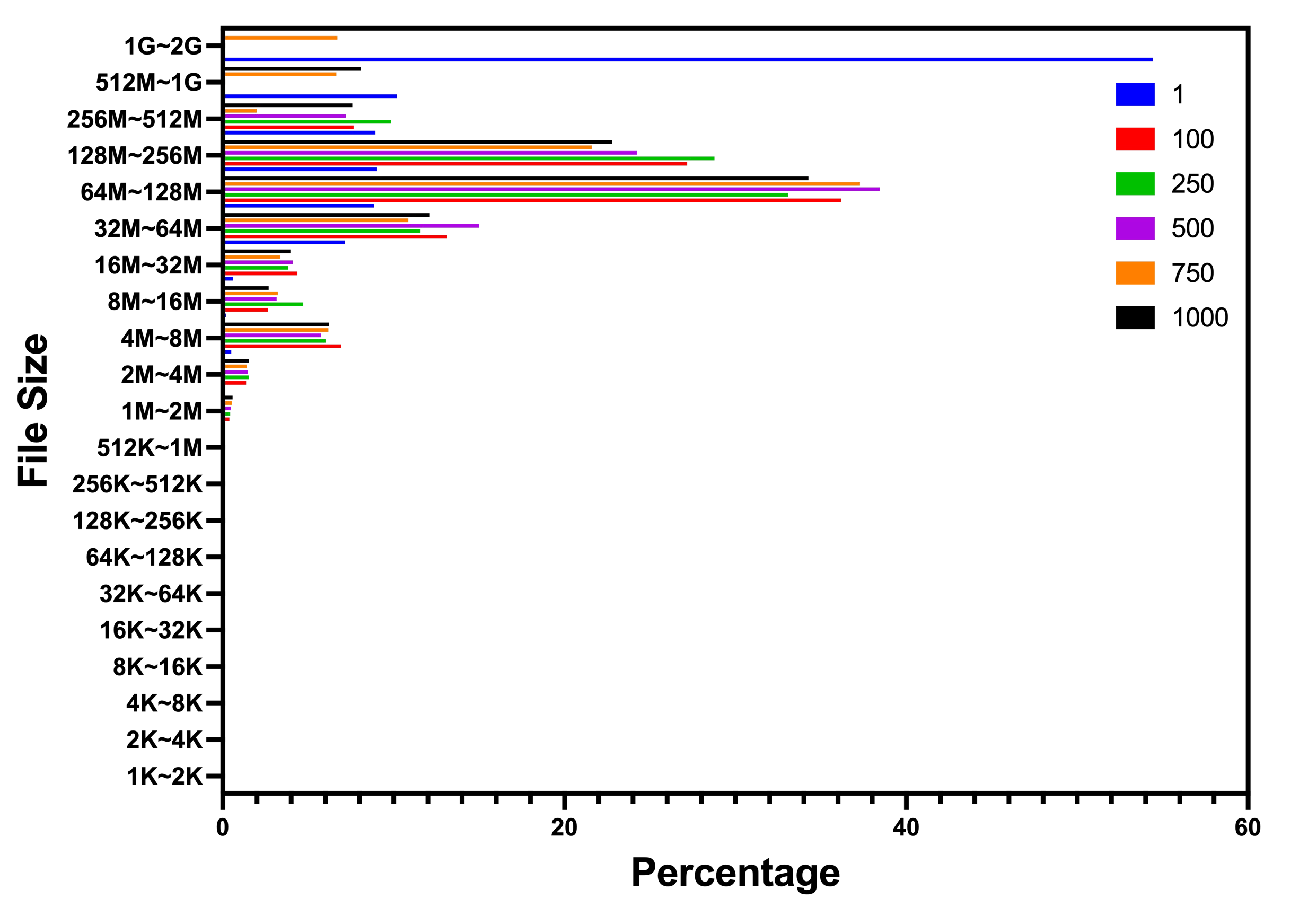
\includegraphics[width=0.95\columnwidth]{free_block_rocksdb}
	\caption{}
	\label{f:}
\end{figure}

\begin{figure}[t]
    \centering
	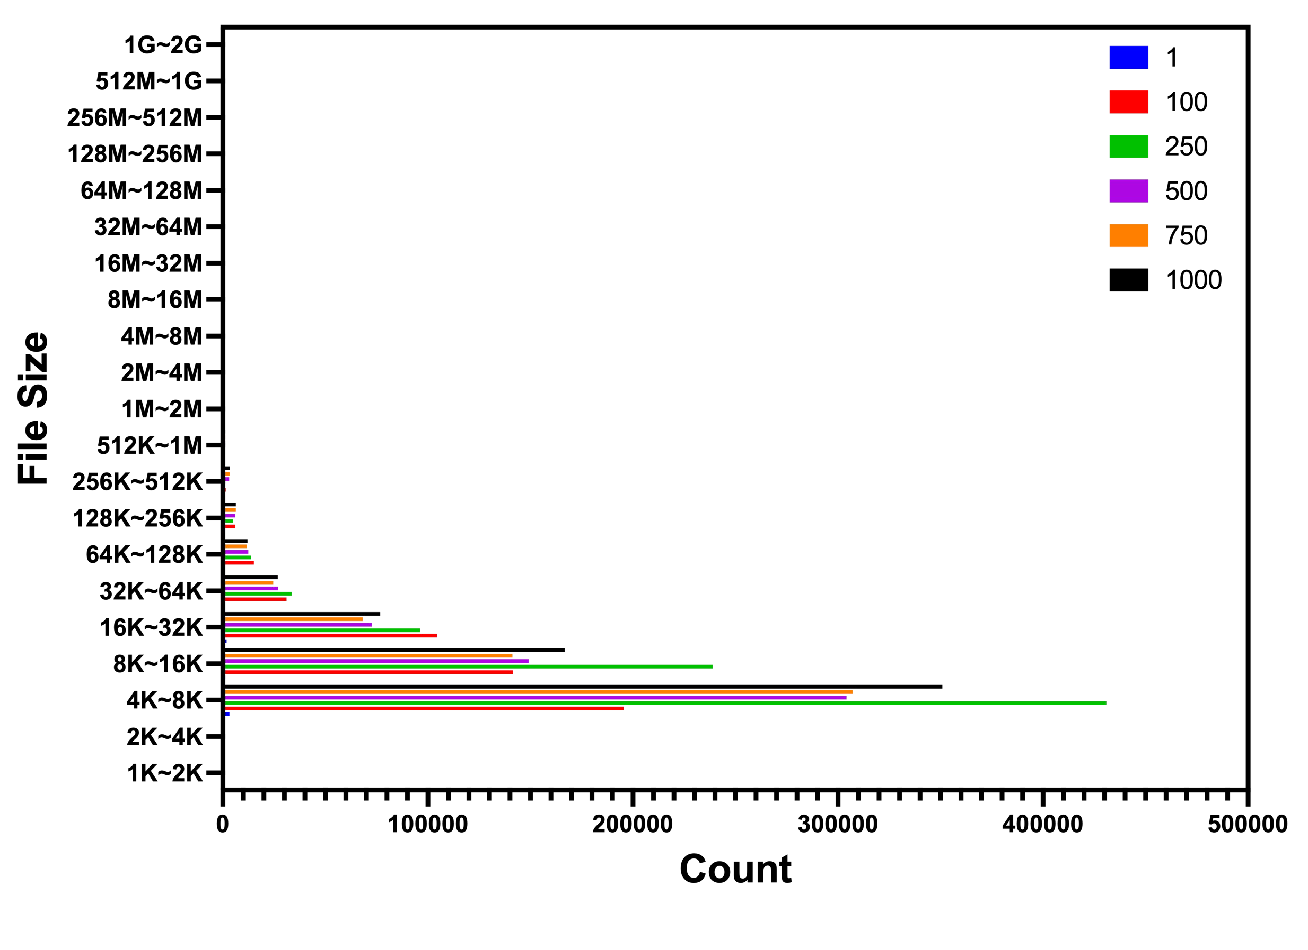
\includegraphics[width=0.95\columnwidth]{free_extents_ext4}
	\caption{}
	\label{f:}
\end{figure}

\begin{figure}[t]
    \centering
	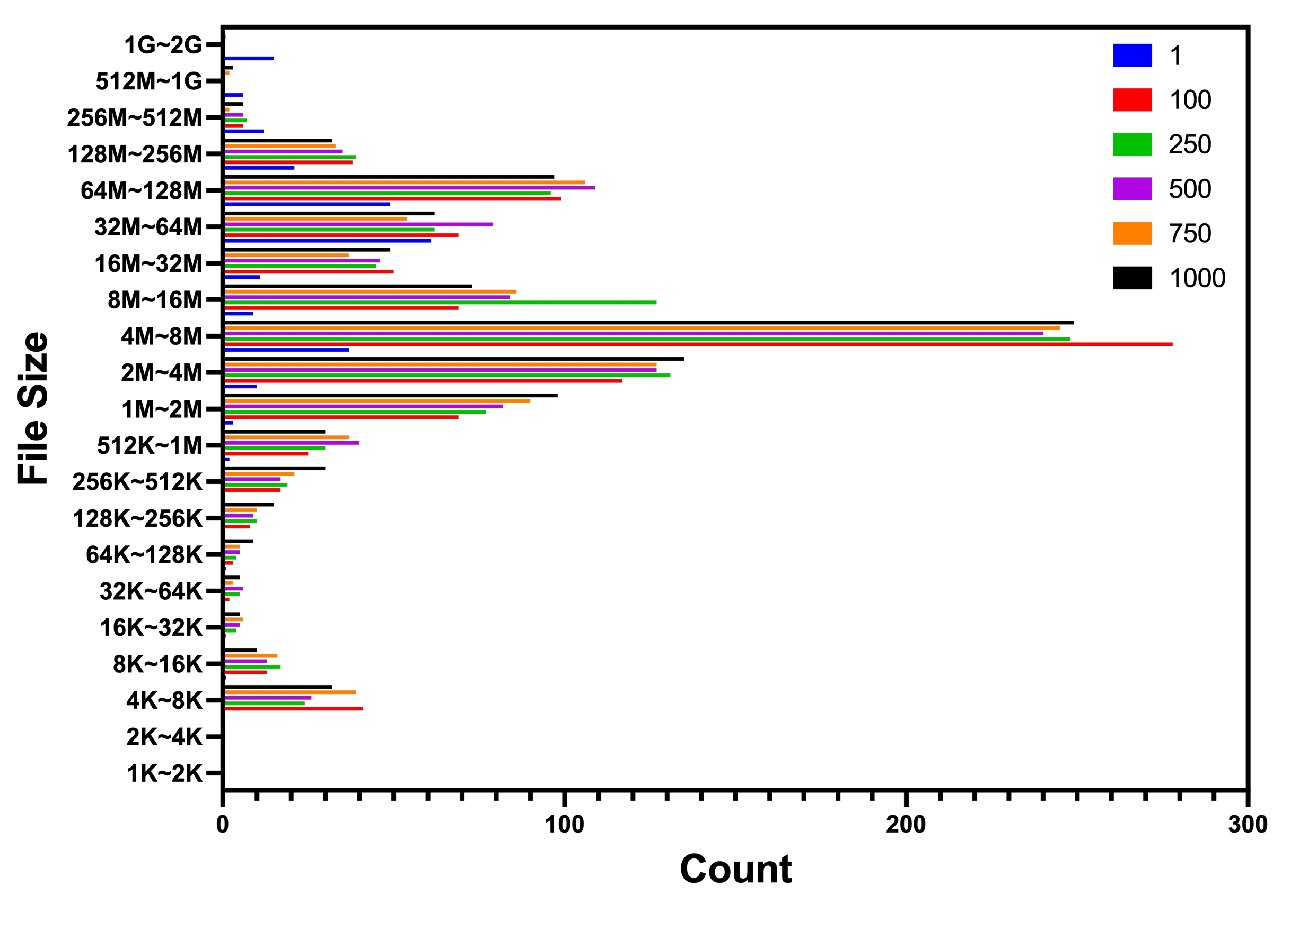
\includegraphics[width=0.95\columnwidth]{free_extents_rocksdb}
	\caption{}
	\label{f:}
\end{figure}

\begin{figure}[t]
    \centering
	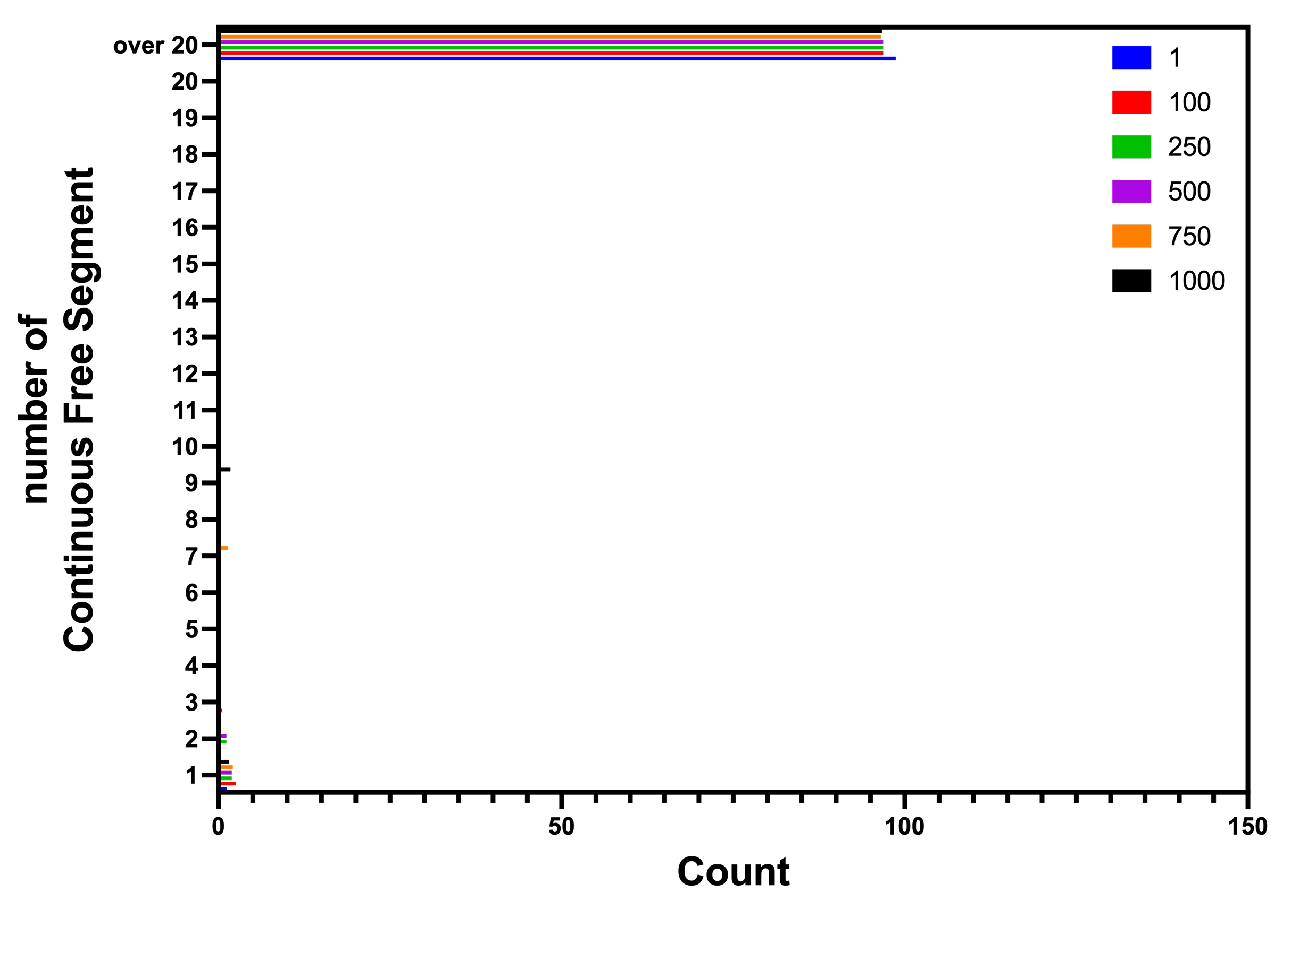
\includegraphics[width=0.95\columnwidth]{free_segment_f2fs}
	\caption{}
	\label{f:}
\end{figure}

\begin{figure}[t]
    \centering
	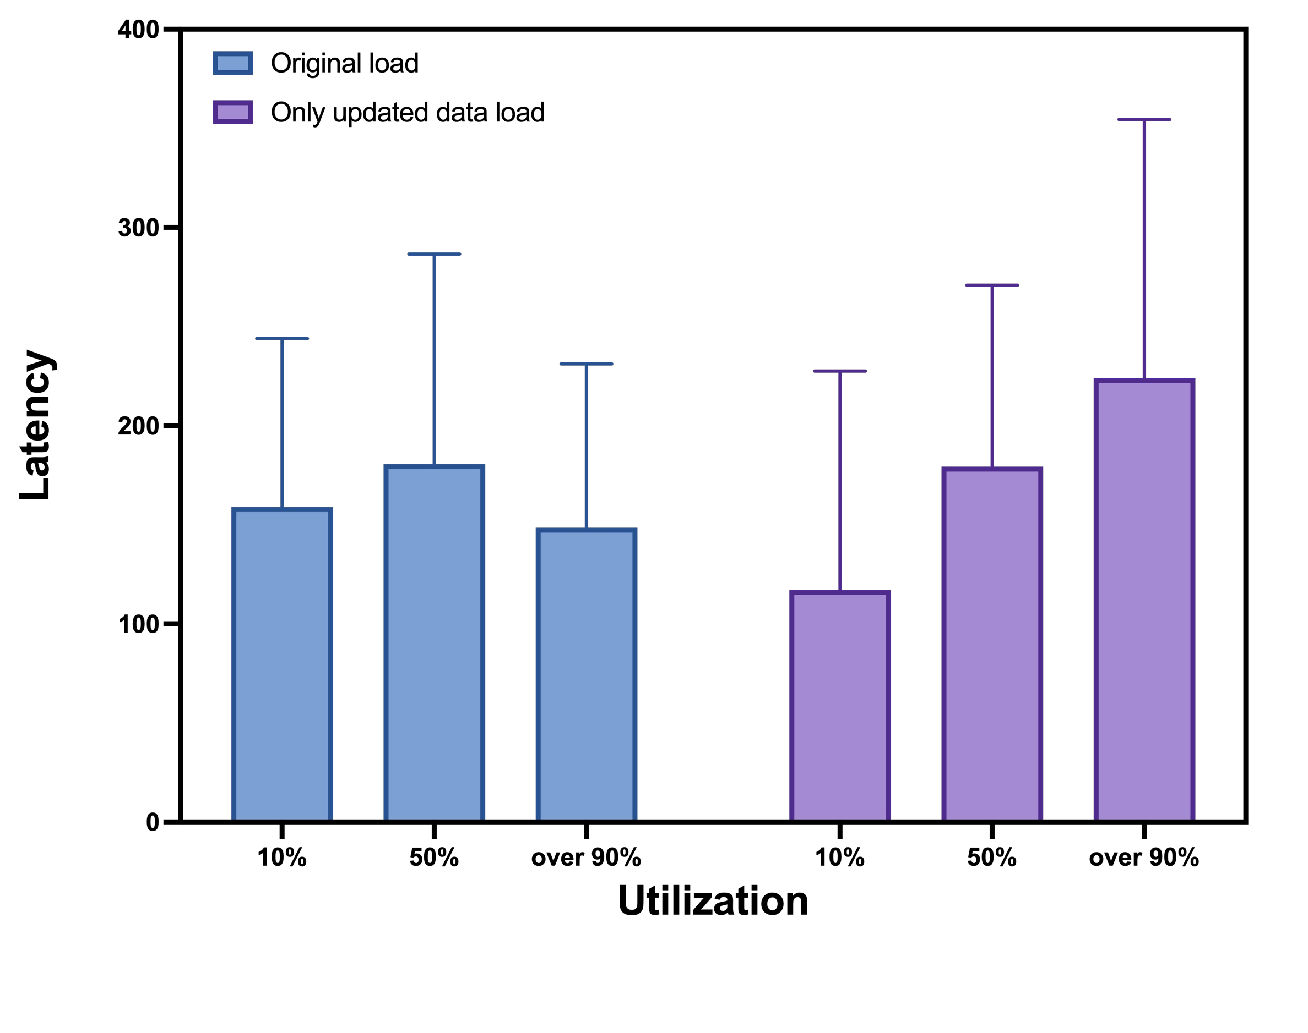
\includegraphics[width=0.95\columnwidth]{load_latency}
	\caption{}
	\label{f:}
\end{figure}

\begin{figure}[t]
    \centering
	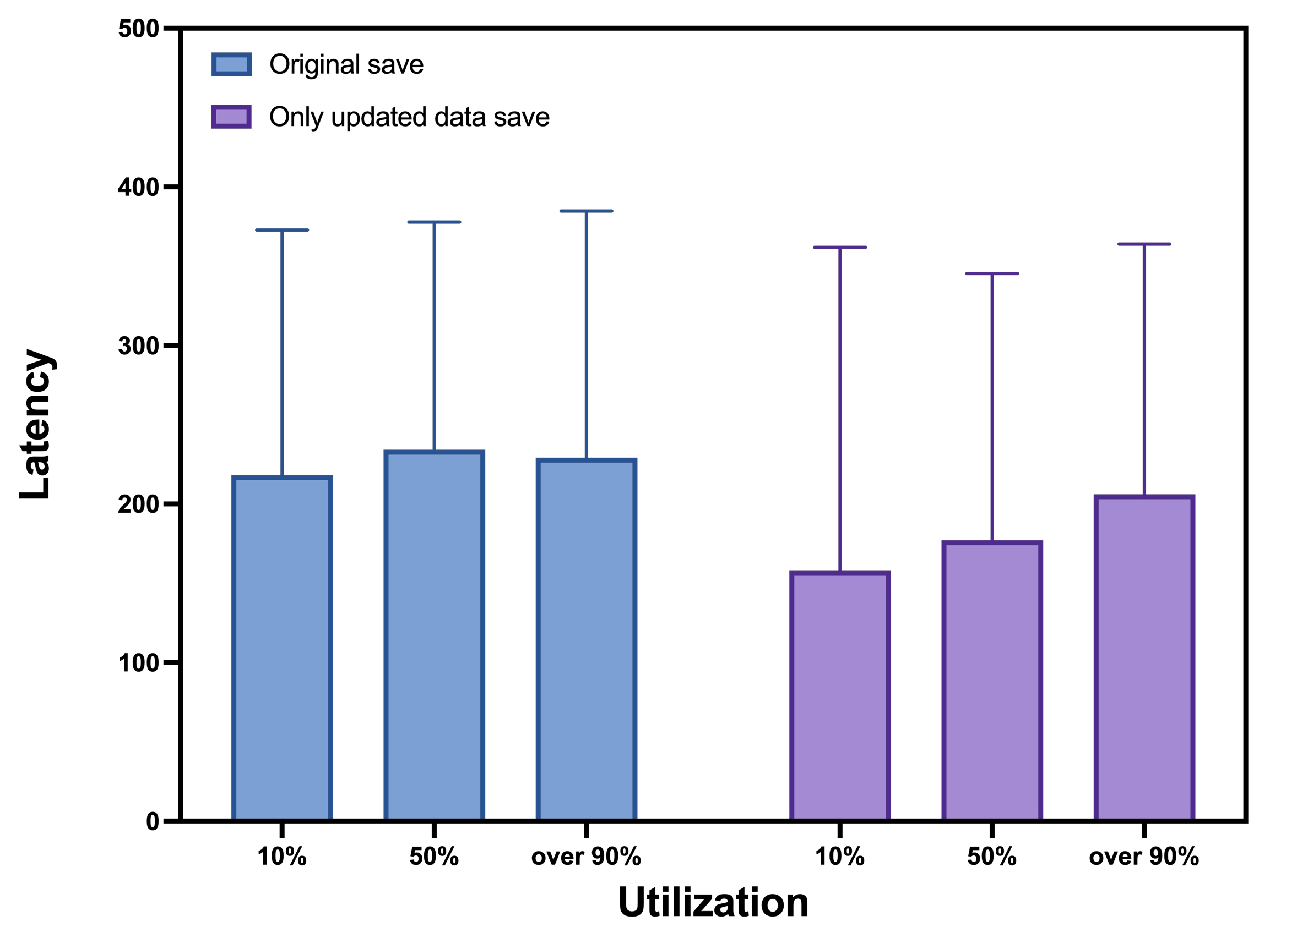
\includegraphics[width=0.95\columnwidth]{save_latency}
	\caption{}
	\label{f:}
\end{figure}
